\chapter{Spatial Early Warning Signals}
\label{chapter:spatial_ews}
\graphicspath{{spatial_ews/figs}}

Earlier in this thesis, specific examples of tipping points were examined.
There is much interest in creating monitoring systems to determine how close these and other tipping points are to being triggered.
One proposed way to do this is with Early Warning Signals. These Early Warning Signals assume the system is forced slowly compared to its timescale.
However in the case of many systems of interest, the forcing (climate change) is fast relative to the system's own dynamics.
In this chapter I will try to produce Early Warning Signals more appropriate to this case.

\section{Fast and Slow Tipping Elements}
An open question in the theory of Early Warning Signals is how to modify them to be appropriate to the case when the control parameter of a system
changes quickly relative to the timescale of the system \parencite{VanderBolt2021}. To formalise what is meant by a control parameter changing rapidly relative
to the system, consider the system
\begin{equation}
  \label{eq:system_with_a_timescale}
  \dv{y}{t} = \frac{f(y,rt)}{T}
\end{equation}
where $y$ is the system state, $T$ is a characteristic timescale of the system and $r$ is the rate the system is linearly forced
at. There is an associated frozen system
\begin{equation}
  \label{eq:system_with_a_timescale_frozen}
  \dv{y}{t} = \frac{f(y,\mu)}{T}
\end{equation}
where $\mu$ is a constant control parameter. Suppose further than there is a bifurcation in the frozen system when
$\mu = \mu^*$, which corresponds to a tipping point in \cref{eq:system_with_a_timescale} at time $t = t^*$ (i.e.\ when the forcing reaches a magnitude of $rt^* = \mu^*$).
By considering the ratio of the system's timescale $T$, to forcing timescale, $1/r$,  the parameter $\epsilon = rT$ can be defined. Time can be rescaled through $t=Ts$
so that \cref{eq:system_with_a_timescale} becomes
\begin{equation}
  \label{eq:system_with_a_timescale_rescaled}
  \dv{y}{s} = f(y,\epsilon s).
\end{equation}

Alternatively this can be rewritten autonomously as
\begin{subequations}
  \label{eq:system_with_a_timescale_rescaled_autonomous}
  \begin{align}
    \dv{y}{s} &= f(y,\mu) \\
    \dv{\mu}{s} &= \epsilon.
  \end{align}
\end{subequations}

An important limit  is the small $\epsilon$ limit. This corresponds to small $r$, which means the system is forced very slowly, or equivalently to
large $T$ --- which means the system responds very slowly to forcing. In this limit \cref{eq:system_with_a_timescale_rescaled_autonomous} is a
fast-slow system \parencite{Kuehn2011} and the usual tools of bifurcation theory can be applied without too much difficulty. In this case,
rises in the autocorrelation and variance of fluctuations about the system's quasi-static equilibrium state are to be expected as the tipping point is approached  \parencite{Scheffer2009}.

In the case of climate change, systems to which this small $\epsilon$ limit applies are known as \emph{fast tipping elements}. An example of a fast tipping element is
the Amazon rainforest \parencite{Ritchie2021}.

There also exist \emph{slow tipping elements} in which $\epsilon$ is not small. It is difficult to get good early warning signals
using the variance and autocorrelation techniques \parencite{VanderBolt2021}. Unfortunately these systems which respond slowly to forcing, such as the Greenland ice
sheet \parencite{Ritchie2021}, are common in the Earth system.

This is because the rate of global warming is fast, on the order of \SI{1}{\kelvin} per century \parencite{Osborn2021}, which is a rate unprecedented in at least
the last 2000 years \parencite{AR6}. Many important tipping elements have timescales of centuries or longer \parencite{Lenton2008,ArmstrongMcKay2022}.
This implies that for tipping elements subject to anthropogenic climate change $\epsilon$ is unlikely to be small, as shown in \cref{tab:epsilon_estimate}.
This motivates the development of Early Warning Signals that are reliable for systems with larger values of $\epsilon$.

\begin{table}
  \centering
  \begin{tabular}{lll}
    \toprule
    Tipping Element                & System Timescale (years) & Estimated $\epsilon$  \\
    \midrule
    Greenland Ice Sheet            & $10000$                  & $200$                 \\
    West Antarctic Ice Sheet       & $2000$                   & $40$                  \\
    Southern Polar Gyre Convection & $10$                     & $0.2$                 \\
    Amazon Rainforest              & $100$                    & $2$                   \\
    Boreal Permafrost              & $50$                     & $1$                   \\
    AMOC                           & $50$                     & $1$                   \\
    \bottomrule
  \end{tabular}
  \caption{Estimates of $\epsilon$ values for a subset of tipping elements using the estimated timescales in~\cite{ArmstrongMcKay2022}.
    The forcing timescale was chosen to be $\SI{50}{\year}$, which corresponds to around $\SI{3}{\kelvin}$ of warming by the end of the century,
    which is about the level of warming expected under current policies \parencite{Rogelj2023}.}
    \label{tab:epsilon_estimate}
\end{table}


One way to understand the problems with Early Warning Signals for slow tipping elements is to recognise that the equilibrium implied by the changing forcing is changing
significantly over the sliding windows used to calculate the Early Warning Indicators. Although it may be possible to make the sliding window shorter, this will
increase the uncertainties on any statistical estimate. Furthermore, the sliding window must be large enough to resolve the critical dynamics of the system which are slowing down
and so tending to be becoming larger than the sliding window. A potential way to avoid this problem is to try to make `instantaneous' measurements of
the variance and autocorrelation of the fluctuations about equilibrium. This could be done by calculating these statistics over space instead of over time.

Spatial early warning signals have been studied before.~\cite{Donangelo2010} compared spatial and temporal early warning signals, finding that the spatial variance
can give an earlier early warning than the temporal variance. Another study \parencite{Kefi2014} found rising memory, variability and changes to patchiness were all
spatial indicators of an upcoming transition. A range of studies have applied spatial early warnings to ecological problems \parencite{Carpenter2010,Dakos2011,Guttal2009}.
Spatial early warning signals have even been applied to observational data \parencite{Tirabassi2023,Kefi2007,Eby2017}. It should be noted that recent high profile applications to
the earth system \parencite{Boulton2022,Boers2021,Boers2021a} have all involved temporal rather than spatial indicators, even though spatially resolved data was used.

\section{The System}
In order to investigate spatial early warning signals a specific system will be examined. This system will be chosen
to be generic enough that broader conclusions can be drawn. The system will be made as simple as possible to aid in the analysis.

As outlined in \cref{sec:btipping} near a B-tipping point many systems are governed by similar one-dimensional dynamics, which motivates the introduction of one dependent
variable $y$. In one dimension there is only one generic type of bifurcation, the saddle node \parencite{Thompson1994}. The saddle node normal form is
$\dot{y} = \mu - y^2$, however $y$ diverges for $\mu < 0$. Therefore to keep $y$ finite and the dynamics simple, the system to be investigated will contain only the lowest order terms
which give a saddle node and bounded dynamics, namely $\dot{y} = y - y^3/3 - \mu$, where $\mu$ is a control parameter.

To take into account the spatial nature of the problem a coupling in space must be considered. Attention will be restricted to a 1 dimensional
periodic domain of length $L$. To couple in space the well studied diffusive coupling is used; this acts to smooth out the value of $y$ over the domain.
Such a diffusive form has found numerous uses in climate and ecological models. For example, it has been used in energy balance models for
the global temperature \parencite{Ghil1976}, ecosystem pattern formation \parencite{Gowda2014,Bastiaansen2018} and in continuum models of the compost bomb \parencite{Clarke2021}.

Noise will be introduced into the system and the control parameter, $\mu$,  will change linearly with time. These considerations combine to motivate studying
\begin{subequations}
\label{eq:spatial_system}
  \begin{align}
    \pdv{y}{t} &= y - \frac{1}{3}y^3 - \mu + D\pdv[2]{y}{x} + \sigma\zeta \label{eq:spatial_system_y} \\
    \dv{\mu}{t}&= \epsilon \label{eq:spatial_system_mu}
  \end{align}
\end{subequations}
where $\zeta$ is delta-correlated noise with mean
\begin{equation}
  \label{eq:delta_mean}
  \E \left[\zeta\left(x,t\right)\right] = 0 
\end{equation}
and covariance
\begin{equation}
  \label{eq:delta_cov}
  \E \left[\zeta\left(x,t\right)\zeta(x',t')\right] = \delta(x-x')\delta(t-t') 
\end{equation}
The parameter $\sigma^2$ is the variance of the noise, and $D$ gives the strength of the spatial coupling.
The variable $\mu$ linearly increases between $\mu = 0$ and $\mu = 1$ and so the system will undergo a saddle node bifurcation at $\mu = 2/3$. \todo{Do a nice plot?}

This system can be viewed variationally\footnote{A brief review of the concepts of the variational derivative are presented in \cref{appendix:variational_calculus}.}.
To do this define the `energy' of the system as
\begin{equation}
  \label{eq:spatial_system_energy}
  \mathcal{E} = \int_0^L -\frac{1}{2}y^2 + \frac{1}{12}y^4 + \mu y + \frac{1}{2}D\left(\pdv{y}{x}\right)^2\,\mathrm{d}{x}.
\end{equation}

This gives further justification for using a diffusive coupling in the following sense. Suppose a general $\mathcal{E}$ was written as a power series
\begin{equation}
  \label{eq:energy_power_series}
  \mathcal{E} = \int_0^L  -\frac{1}{2}y^2 + \frac{1}{12}y^4 + \mu y + b_1 \pdv{y}{x} + b_2 y \pdv{y}{x} + b_3 \left(\pdv{y}{x}\right)^2 + \ldots \dd{x}.
\end{equation}
If the coupling is required to be isotropic in space, then $b_1 = b_2 = 0$, so to lowest order \cref{eq:energy_power_series} reduces to
\cref{eq:spatial_system_energy}.

Given $\mathcal{E}$ \cref{eq:spatial_system_y} can be rewritten as
\begin{equation}
  \label{eq:spatial_system_y_variational}
    \pdv{y}{t} = -\fdv{\mathcal{E}}{y(x)}  + \sigma\zeta, 
\end{equation}
which is a Time Dependent Ginzburg Landau equation which describes the mean field dynamics of systems like the Ising model \parencite{Goldenfeld1992}.

\section{The Effect of Diffusion on Critical Slowing Down}
\label{sec:spatial_csd}
In \cref{sec:introduction} it was shown how critical slowing down leads temporal early warning signals. In this section, I will show that early warning signals are still expected
to manifest themselves when viewed spatially. Recognising that \cref{eq:spatial_system_y_variational} describes the mean field dynamics of
the Ising model, I will do this using the results of the Landau theory of phase transitions. To draw connections between this and critical slowing down in non-spatial systems
I will begin by calculating the early warning indicators using a Fokker-Planck approach for the uncoupled case.

The uncoupled case corresponds to  $D = 0$. Furthermore, assume $\epsilon$ is small enough so that $\mu$ can be taken to be a parameter of the system.
This is equivalent to calculating the conventional early warning signals over an ensemble of realisations and so should reproduce the well known results about rising variance
and autocorrelation \parencite{Dakos2008}.

Linearising the system about an equilibrium, $y^*$, gives
\begin{equation}
  \label{eq:linearised_spatial}
  \dv{z}{t} = -\lambda z + \sigma \zeta
\end{equation}
where $z = y - y^*$ and $\lambda = (y^*)^2 - 1$. 
In this case, the Fokker-Planck equation, \cref{eq:fokker_planck}, can be used to calculate the statistics \parencite{Risken1984}.
The Fokker-Planck equation associated with \cref{eq:linearised_spatial} is
\begin{equation}
  \label{eq:fokker_planck_linearised_spatial}
  \pdv{p}{t} = \pdv{z}\lambda z p + \frac{1}{2}\sigma^2 \pdv[2]{p}{z}
\end{equation}
where $p$ is the pdf for the system. The steady state solution, assuming $p$ and its derivatives vanish as $z\rightarrow \pm\infty$ is
\begin{equation}
  \label{eq:solution_to_fokker_planck}
  p(z) = \frac{1}{Z} e^{-\frac{1}{\sigma^2}\lambda z^2}.
\end{equation}
The normalisation factor $Z$ is given by
\begin{equation}
  \label{eq:partition_function}
  Z = \int_{-\infty}^{\infty} e^{-\frac{1}{\sigma^2}\lambda z^2} \dd{z} = \frac{\sigma}{\sqrt{\lambda}} \sqrt{\pi}.
\end{equation}
Note that the variance of $z$ is
\begin{equation}
  \label{eq:var_z}
  \sigma_z^2 = -\sigma^2 \pdv{\log Z}{\lambda} = \frac{\sigma^2}{ 2\lambda}
\end{equation}
so that as $\lambda \rightarrow 0$ as the system moves towards the bifurcation it will be the case that $\sigma_z^2$ diverges.
It follows from the Fluctuation-Dissipation Theorem \parencite{Marconi2008} that the autocorrelation at lag-$t$ is $\alpha(t) = e^{-\lambda t}$ and so $\alpha \rightarrow 1$ at the bifurcation.
This is the same behaviour as in the non-spatial case, as expected.

If $D \neq 0$, then \cref{eq:linearised_spatial} becomes
\begin{equation}
  \label{eq:linearised_spatial_D}
  \pdv{z}{t} = -\lambda z + D \pdv[2]{z}{x} + \sigma\zeta = -\fdv{\mathcal{H}}{z} + \sigma \zeta,
\end{equation}
where
\begin{equation}
  \label{eq:linearised_energy}
  \mathcal{H} = \int_0^L \frac{1}{2}\lambda z^2 + \frac{1}{2}D\left(\pdv{z}{x}\right)^2 \dd{x}.
\end{equation}
\Cref{eq:linearised_spatial_D} can be analysed by performing a Fourier series decomposition \parencite{riley2006}, where a function $q(x,t)$ can be split
into oscillatory modes in space with amplitude $q_k(t)$ for wavenumber $k$ defined through
\begin{equation}
  \label{eq:fourier}
  q(x,t) = \frac{1}{L} \sum_k q_k(t) e^{ikx}
\end{equation}
where $q_k = q_{-k}^*$ to ensure that $q(x,t) \in \mathbb{R}$.
Performing this decomposition gives an equation for each mode
\begin{equation}
  \label{eq:linearised_spatial_D_modes}
  \dv{z_k}{t} = -\lambda z_k - Dk^2 z_k + \sigma \zeta_k
\end{equation}
Each mode with wavenumber $k$ therefore relaxes to equilibrium on a timescale
\begin{equation}
  \label{eq:equilirium_timescale}
  \tau_k = \frac{1}{\lambda + Dk^2}.
\end{equation}
As $\lambda \rightarrow 0$, then $\tau_k$ increases, so critical slowing down is still to be expected. Suppose however that only large $k$ modes were resolved, which corresponds to
viewing the system at too small a scale. In this case $\tau_k \sim 1/Dk^2$ so critical slowing down would not be observed until $\lambda$ becomes small enough, which would hamper early
warning signals.

To investigate the effects of critical slowing down on variance and autocorrelation, the probability distribution, $p[z,t]$ which is now a functional of $z$,
of \cref{eq:linearised_spatial_D} must be calculated. This system has its own
form of the Fokker-Planck equation \parencite{Goldenfeld1992} which describes the evolution of $p[z,t]$,
\begin{equation}
  \label{eq:fokker_planck_functional}
  \pdv{p}{t} = \int \fdv{z(x')} \left( \pdv{\mathcal{H}}{z(x')} p + \frac{1}{2}\sigma^2 \fdv{p}{z(x')}\right) \dd{x'}.
\end{equation}
Again, this has an equilibrium solution
\begin{equation}
  \label{eq:fokker_planck_functional_equilibrium}
  p[z,t] = \frac{1}{Z} e^{-\frac{2}{\sigma^2} \mathcal{H}[z]}
\end{equation}
where
\begin{equation}
  \label{eq:partition_functional}
  Z = \int e^{-\frac{2}{\sigma^2} \mathcal{H}[z]}\,\mathcal{D}z.
\end{equation}

In order to find the variance, consider the two-point correlation function
\begin{equation}
  \label{eq:two_point_corr}
  G(x_1 - x_2) = \E \left(z\left(x_i\right)z\left(x_j\right)\right).
\end{equation}
This function can be obtained by differentiation. After introducing the extra term $-B(x)z(x)$ inside the integral in \cref{eq:linearised_energy}, the two point correlation function
can be shown \parencite{Goldenfeld1992} to be equal to
\begin{equation}
  \label{eq:two_point_from_partition}
  G(x_1-x_2) = \frac{\sigma^2}{4}\fdv{B(x_1)}\fdv{\log Z}{B(x_2)} \eval_{B=0}
\end{equation}
or
\begin{equation}
  \label{eq:two_point_correlation_actual}
  G(x) = \frac{1}{2} \sigma^2 \frac{\xi}{D} e^{-x/\xi}
\end{equation}
where $\xi = \sqrt{D/\lambda}$ is the correlation length. The variance is thus $G(0) = 1/\sqrt{4\lambda D}$, which diverges as the bifurcation is approached.
\section{Statistics}
The autocorrelation and variance of \cref{eq:spatial_system} will be compared when calculated over space and over time. These two different ways of calculating the statistics  will now
be defined. A summary is given in \cref{tab:ews_space_time_definition}.

\subsection{Spatial Statistics}

The average of a quantity, $A$, calculated over space is defined to be
\begin{equation}
  \label{eq:definition_of_average}
  \langle A \rangle = \frac{1}{L}\int_0^L A(y(x,t),x) \,\mathrm{d}x.
\end{equation}
The spatial variance of $y$ at time $t$ is then
\begin{equation}
  \label{eq:spatial_variance}
  \sigma_s(t)^2 = \langle y^2 \rangle - \langle y \rangle^2,
\end{equation}
and the autocorrelation over space is defined as
\begin{equation}
  \label{eq:spatial_autocorrelation}
  \alpha_s(t) = \frac{\langle y(t,x)y(t+\Delta t,x) - \langle y(t,x)^2 \rangle }{\sigma_s(t)^2}.
\end{equation}
The quantity $\Delta t$ is the lag of the autocorrelation. However \cref{eq:spatial_system} will ultimately be solved numerically and
in everything that follows $\Delta t$ will be set to the timestep, so that $\alpha_s$ is the lag-1 autocorrelation.

\subsection{Temporal Statistics}
When working over time, the spatio-temporal data will be converted to temporal data by first averaging in space to get $\left\langle y \right\rangle$.
Averaging in time is defined as follows. Consider the quantity $B(t)$. The temporal average is
\begin{equation}
  \label{eq:definition_of_temporal_average}
  \overline{B} = \frac{1}{T_w}\int_0^{T_w}B(t)\,\mathrm{d}t
\end{equation}
where the average is taken over some suitable window of length $T_w$.

When computing early warning indicators over time, the timeseries must first be `detrended'. The detrended timeseries of $\langle y \rangle$ is denoted by $z$.
The variance and autocorrelation, defined over a window of length $\tau_w$ are
\begin{equation}
  \label{eq:temporal_variance}
  \sigma_t^2 = \overline{z^2} - \overline{z}^2 
\end{equation}
and
\begin{equation}
  \label{eq:temporal_autocorrelation}
  \alpha_t = \frac{\overline{z(t)z(t+\Delta t)}}{\sigma_t^2}.
\end{equation}
\begin{table}
  \centering
  \begin{tabular}{llll}
    \toprule
    Quantity        & Domain & Symbol        & Definition \\
    \midrule
    Variance        & Space  & $\sigma_s^2$  & $\langle y^2 \rangle - \langle y \rangle$ \\
    \rule{0pt}{4ex}    
                    & Time   & $\sigma_t^2$  & $\overline{z^2} - \overline{z}^2$ \\
    \rule{0pt}{4ex}    
    Autocorrelation & Space  & $\alpha_s$    & $\frac{\left\langle y\left(t,x\right)y\left(t+\Delta t,x\right)\right\rangle - \left\langle y\left(t,x\right)^2 \right\rangle}{\sigma_s(t)^2}$ \\
    \rule{0pt}{4ex}    
                    & Time   & $\alpha_t$    &  $\frac{\overline{z(t)z(t+\Delta t)}}{\sigma_t^2}$ \\
    \bottomrule
  \end{tabular}
  \caption[Definition of spatial and temporal early warning signals]{The definition of the early warning indicators used in this chapter, taken from
  \cref{eq:spatial_variance,spatial_autocorrelation,temporal_variance,temporal_autocorrelation}.}
  \label{tab:ews_space_time_definition}
\end{table}

\section{Numerical Results}
\subsection{Numerical Method}
To solve \cref{eq:spatial_system}, the domain, of length $L = 2\pi$, was discretised into $N = 100$ grid
points and 
the diffusive term is calculated with finite differences. The value of $y$ at the $k$th gridpoint is $y_k$. Integration forward in time was accomplished by 
using an implicit Euler method, where the resulting nonlinear equation was solved using 
MINPACK's HYBRD method accessed through SciPy \parencite{Virtanen2020}. To avoid excessively long integrations when $\epsilon$ is small,
the timestep was set to $\delta t = 0.001/\epsilon$ and the system was integrated until $t=1/\epsilon$. Early warning signals were calculated
from $\epsilon t=0$ until $\epsilon t=2/3$, which is the 
time of the tipping point. When working over time, the window size was chosen to 
contain 500 data points (i.e.\ half the time series),
so that the window length is $\tau_w = 1/(2\epsilon)$. Detrending was accomplished by removing a fitted quadratic polynomial from these windows.
To stand a chance of getting good early warning
signals in time it is required that $\epsilon < 1/\tau_w$, which is always satisfied.
Systems are initialised in equilibrium and spun up for 1000 time steps.

\subsection{Two Limits}
Before determining the reliability of the early warning signals as a function of $\epsilon$ and $D$, two important limits will be investigated. They are the uncoupled ($D = 0$)
and slowly forced ($\epsilon \ll 1$) limits.

\subsubsection{Uncoupled Limit}
First the case  when $D = 0$ is investigated, for large and small values of $\epsilon$. Consider \cref{fig:uncoupled_timeseries}.
\begin{figure}
  \centering
  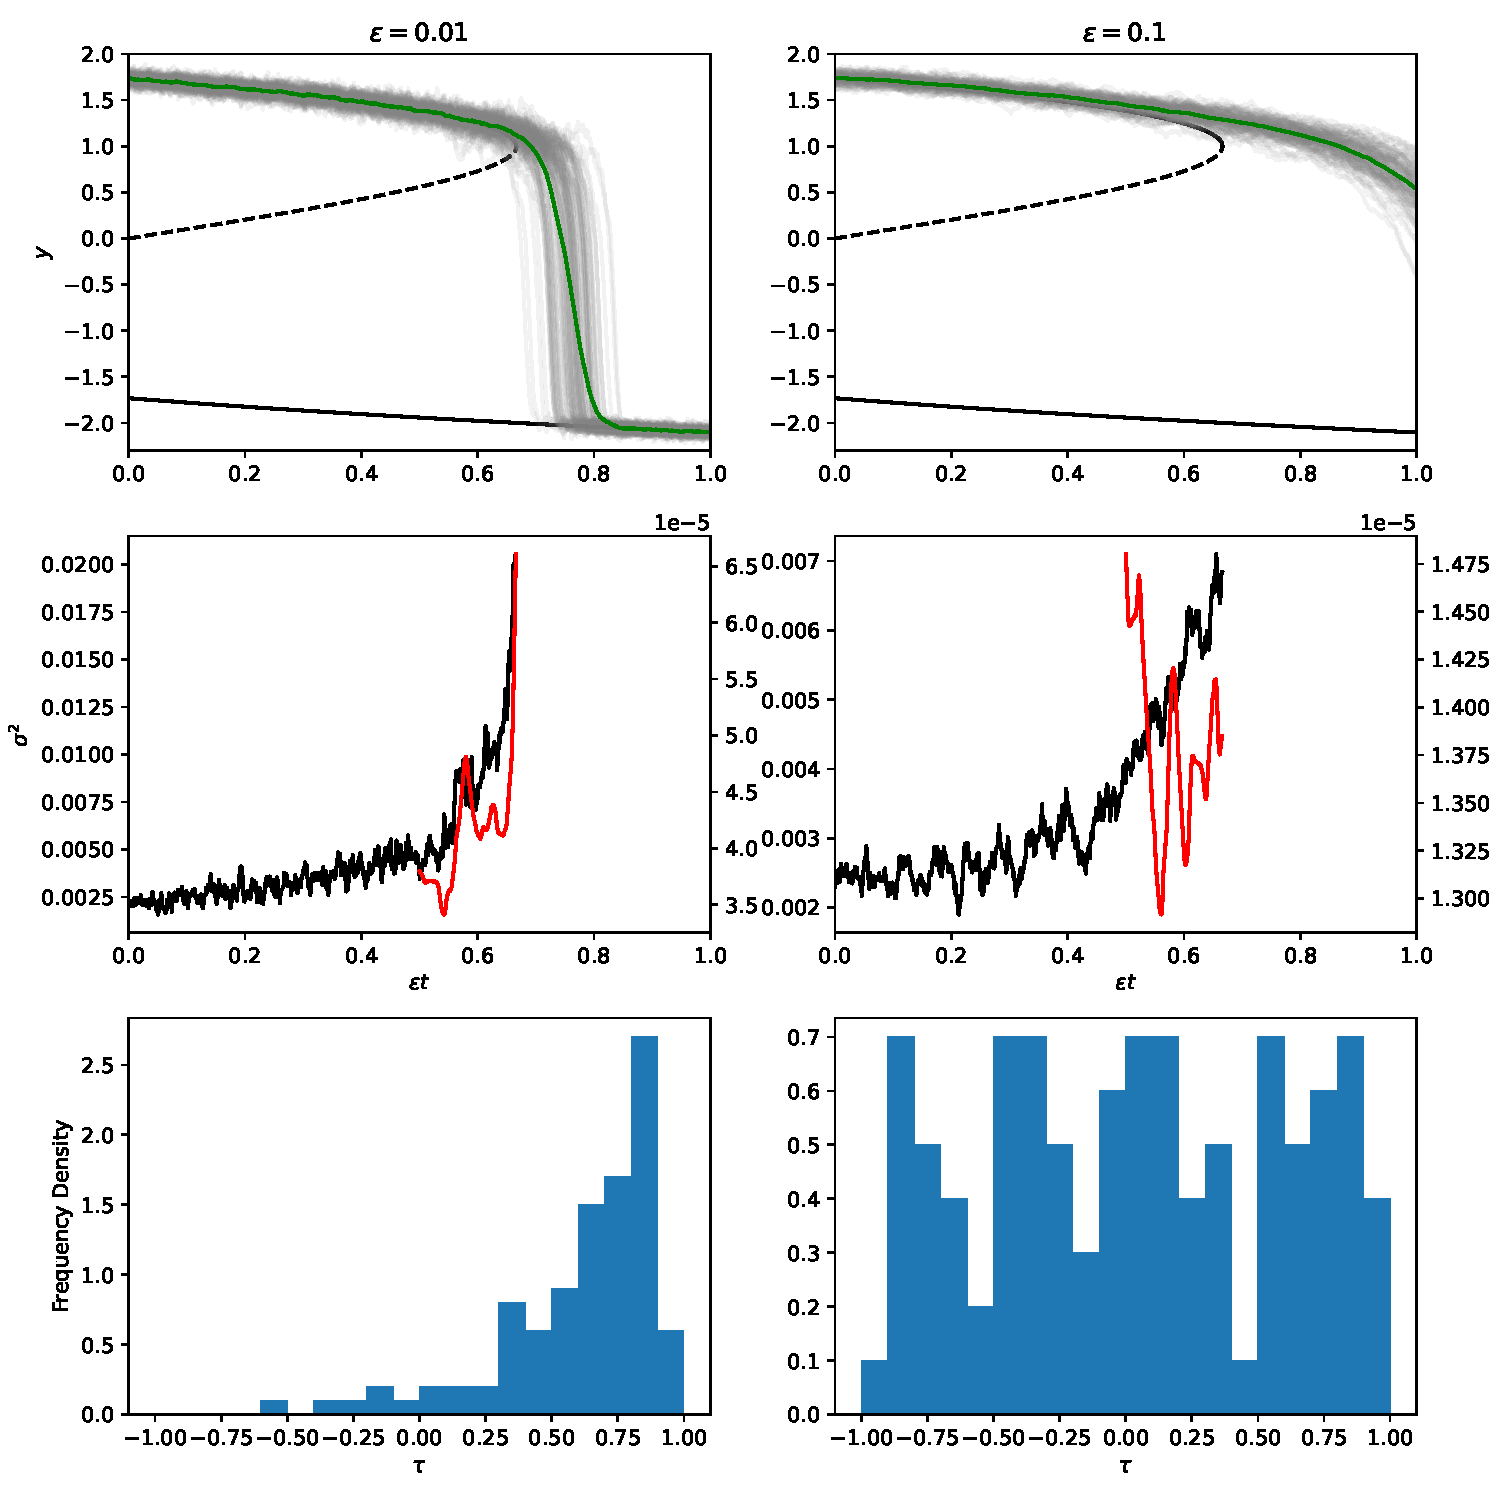
\includegraphics[width=\textwidth,keepaspectratio]{uncoupled_variance}
  \caption[Early warning signals in the uncoupled limit]{Early warning signals when $D = 0$. The left column shows the slow forcing case and the right column shows the fast forcing.
    The top row shows the individual trajectories with the mean trajectory shown in green. The black curves are the quasi-static equilibria.
    In the second row  $\sigma_s^2$ in black and $\sigma_t^2$ in red are plotted. In the bottom row $\sigma_t^2$ is calculated from the individual gridpoints
    rather than the domain average.  The Kendall $\tau$ value is calculated for each gridpoint and then a histogram of these $\tau$ values is plotted. The mean $\tau$ values
    are 0.6 and 0.04 for the slow and fast case respectively.}
  \label{fig:uncoupled_timeseries}
\end{figure}
The left column shows the small $\epsilon$ case. This is the case
where temporal early warning signals are expected to work well. For this value of $\epsilon$ the system
transitions to its new state near the time of the bifurcation and its variance calculated over
space and calculated over time both clearly increase near the bifurcation point. Furthermore
calculating the statistics for each the individual grid points shows that most grid points 
experience a rise in variance over time as well.

For the larger $\epsilon$ case the results are different. The system has not yet transitioned to
its new state even by the end of the simulation. A clear rise in $\sigma_t^2$ cannot be seen near the bifurcation point. Furthermore looking at the individual grid points,
no coherent warning of the upcoming transition is given. However there is a very clear rise in $\sigma_s^2$ before the bifurcation, demonstrating that spatial early warning
signals are superior in this case.

\subsubsection{Slowly Forced Limit}
\Cref{fig:coupled_timeseries} is similar to \cref{fig:uncoupled_timeseries} expect it now examines the limit of slow forcing ($\epsilon = 0.01$) but
but with a non-zero coupling in space. $D$ values of $D = 1$ and $D = 10^5$ were chosen. For low $D$ and slow forcing early warning signals are expected to work both when calculated spatially or
temporally. At higher $D$ the correlations between the grid points will be so great that there will no longer be any variability between different grid points, and so no detection
of spatial early warning signals should be possible. This is precisely what is seen in \cref{fig:coupled_timeseries} where for $D=10^5$ the system acts like a single grid point.
\begin{figure}
  \centering
  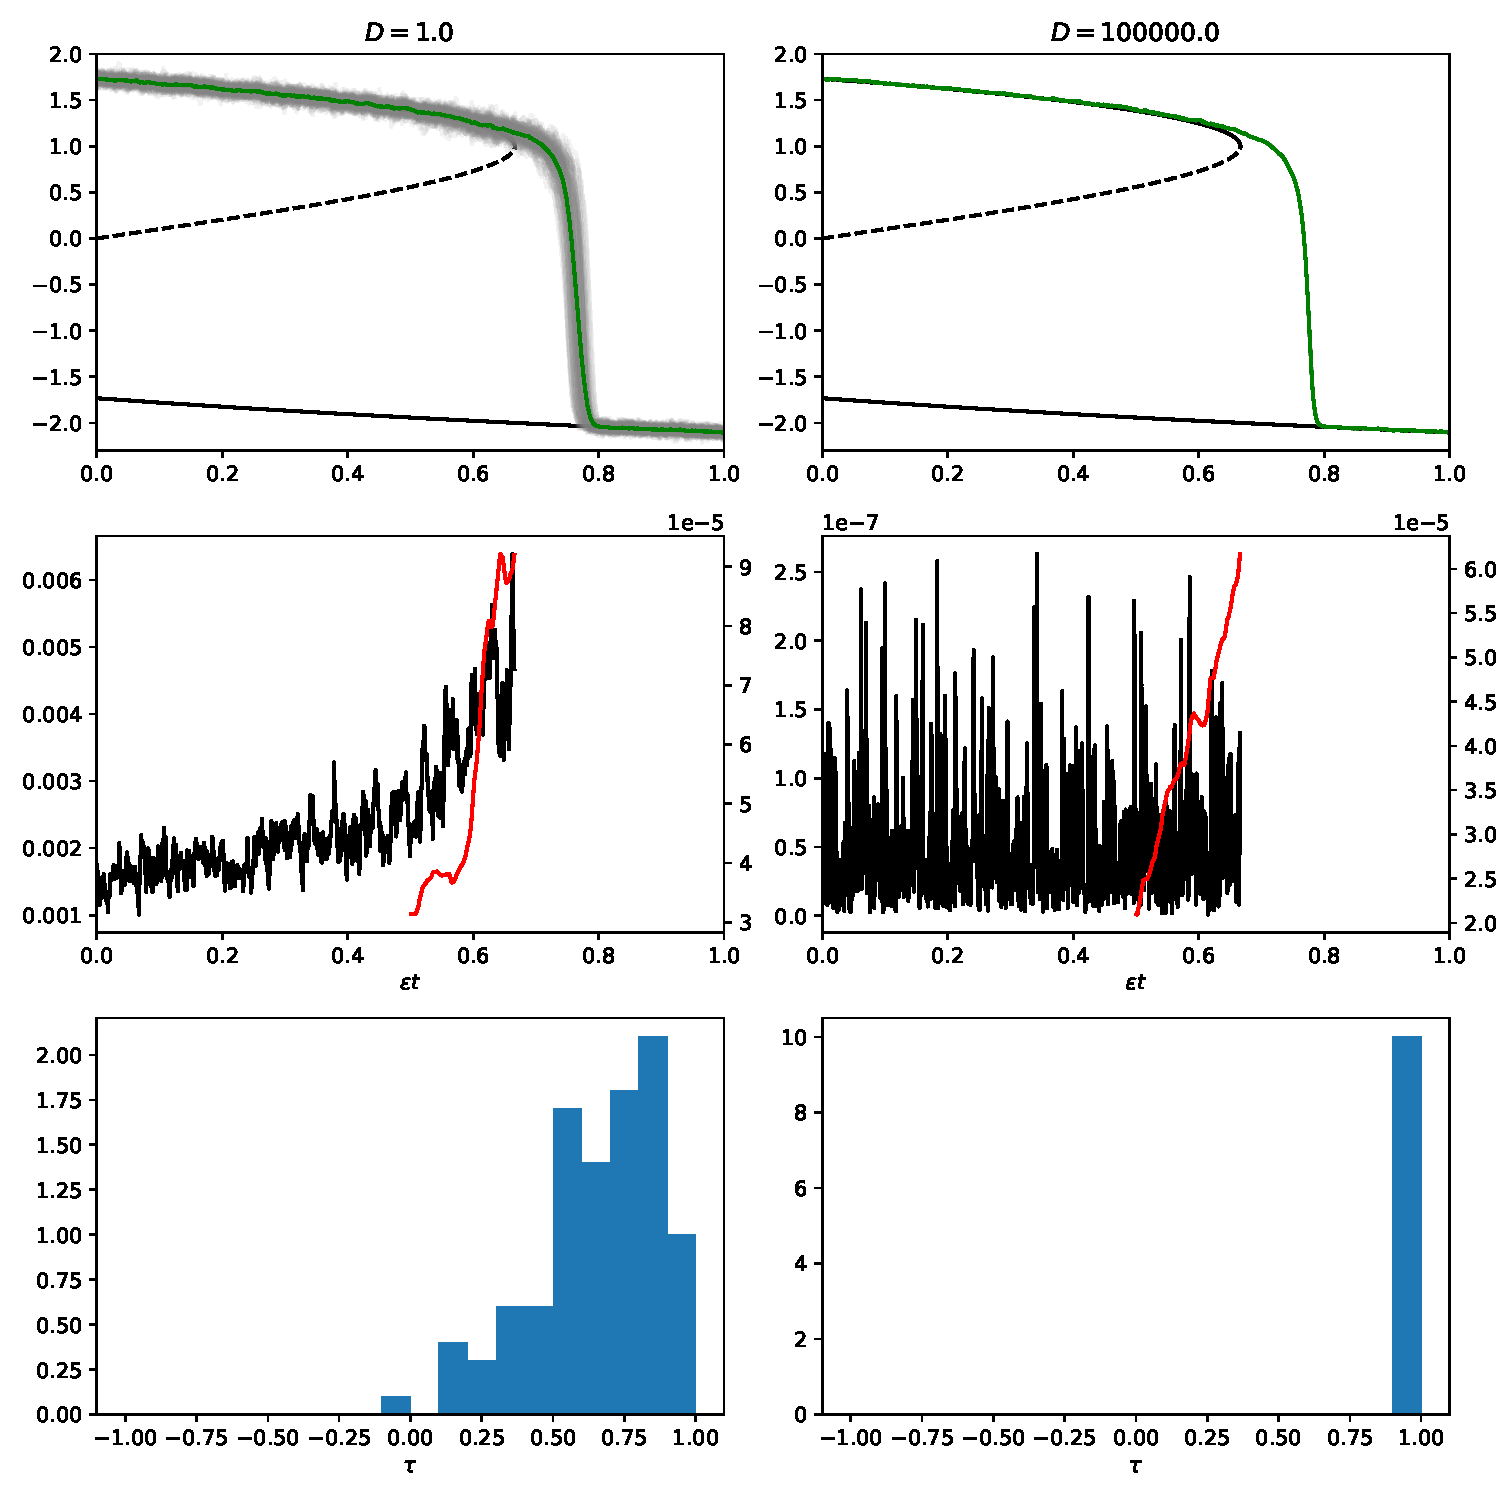
\includegraphics[width=\textwidth,keepaspectratio]{coupled_variance}
  \caption[Early Warning Signals in the slowly forced limit]{Early warning signals when $\epsilon = 0.01$. The left column shows 
    the weakly coupled case, the right shows what happens in the strongly coupled (large $D$) case. 
    The top row shows the quasi-static equilibria (black) the individual
    trajectories of the grid boxes (grey) and the domain average (green).
    The variance is plotted in the second row, calculated over space 
    (black) and over time (red). The bottom row shows a histogram of the Kendall $\tau$ values calculated over time for each $y_k$.}
  \label{fig:coupled_timeseries}
\end{figure}

\subsection{Exploring the $\epsilon$ and $D$ parameter space}
Now that the two limits have been investigated, the parameter space can be explored more fully.
Early warning signals will be investigated in the region of the parameter plane defined by $(\epsilon,\left(\frac{N}{L}\right)^2 D) \in [10^{-2},10^1] \times [10^{-7}, 10^{7}]$.
50 points are sampled in each direction, geometrically spaced, giving $2500$ total points.

It can be determined if an early warning indicator is increasing or decreasing by calculating the Kendall's $\tau$ for the data.
A positive value implies an increasing trend \parencite{Wilks2011}. The reliability of the warning can be assessed by repeating the numerical
experiment 100 times (with different realisations of the noise) and calculating a distribution of Kendall's $\tau$. If the signal-to-noise ratio
(SNR) of the distribution of $\tau$ values, defined as the ratio of the mean to the standard deviation, is smaller than 1 then a reliable early warning cannot be expected.

This signal-to-noise ratio is calculated in \cref{fig:parameter_plane} for temporal and spatial early warning statistics. Only for
certain regions of the parameter plane are early warning signals of the upcoming tipping point reliable. It can be noted that there is a complementarity between spatial
and temporal early warning signals. For rapidly forced systems good early warning signals in space are obtained as long the
the coupling in space is not too strong. Conversely, for strongly coupled systems there are good early warning in time as long the forcing is slow enough. It is important to note that
the strongly coupled and rapidly forced region does not give good early warning signals with either method.

\begin{figure}
  \centering
  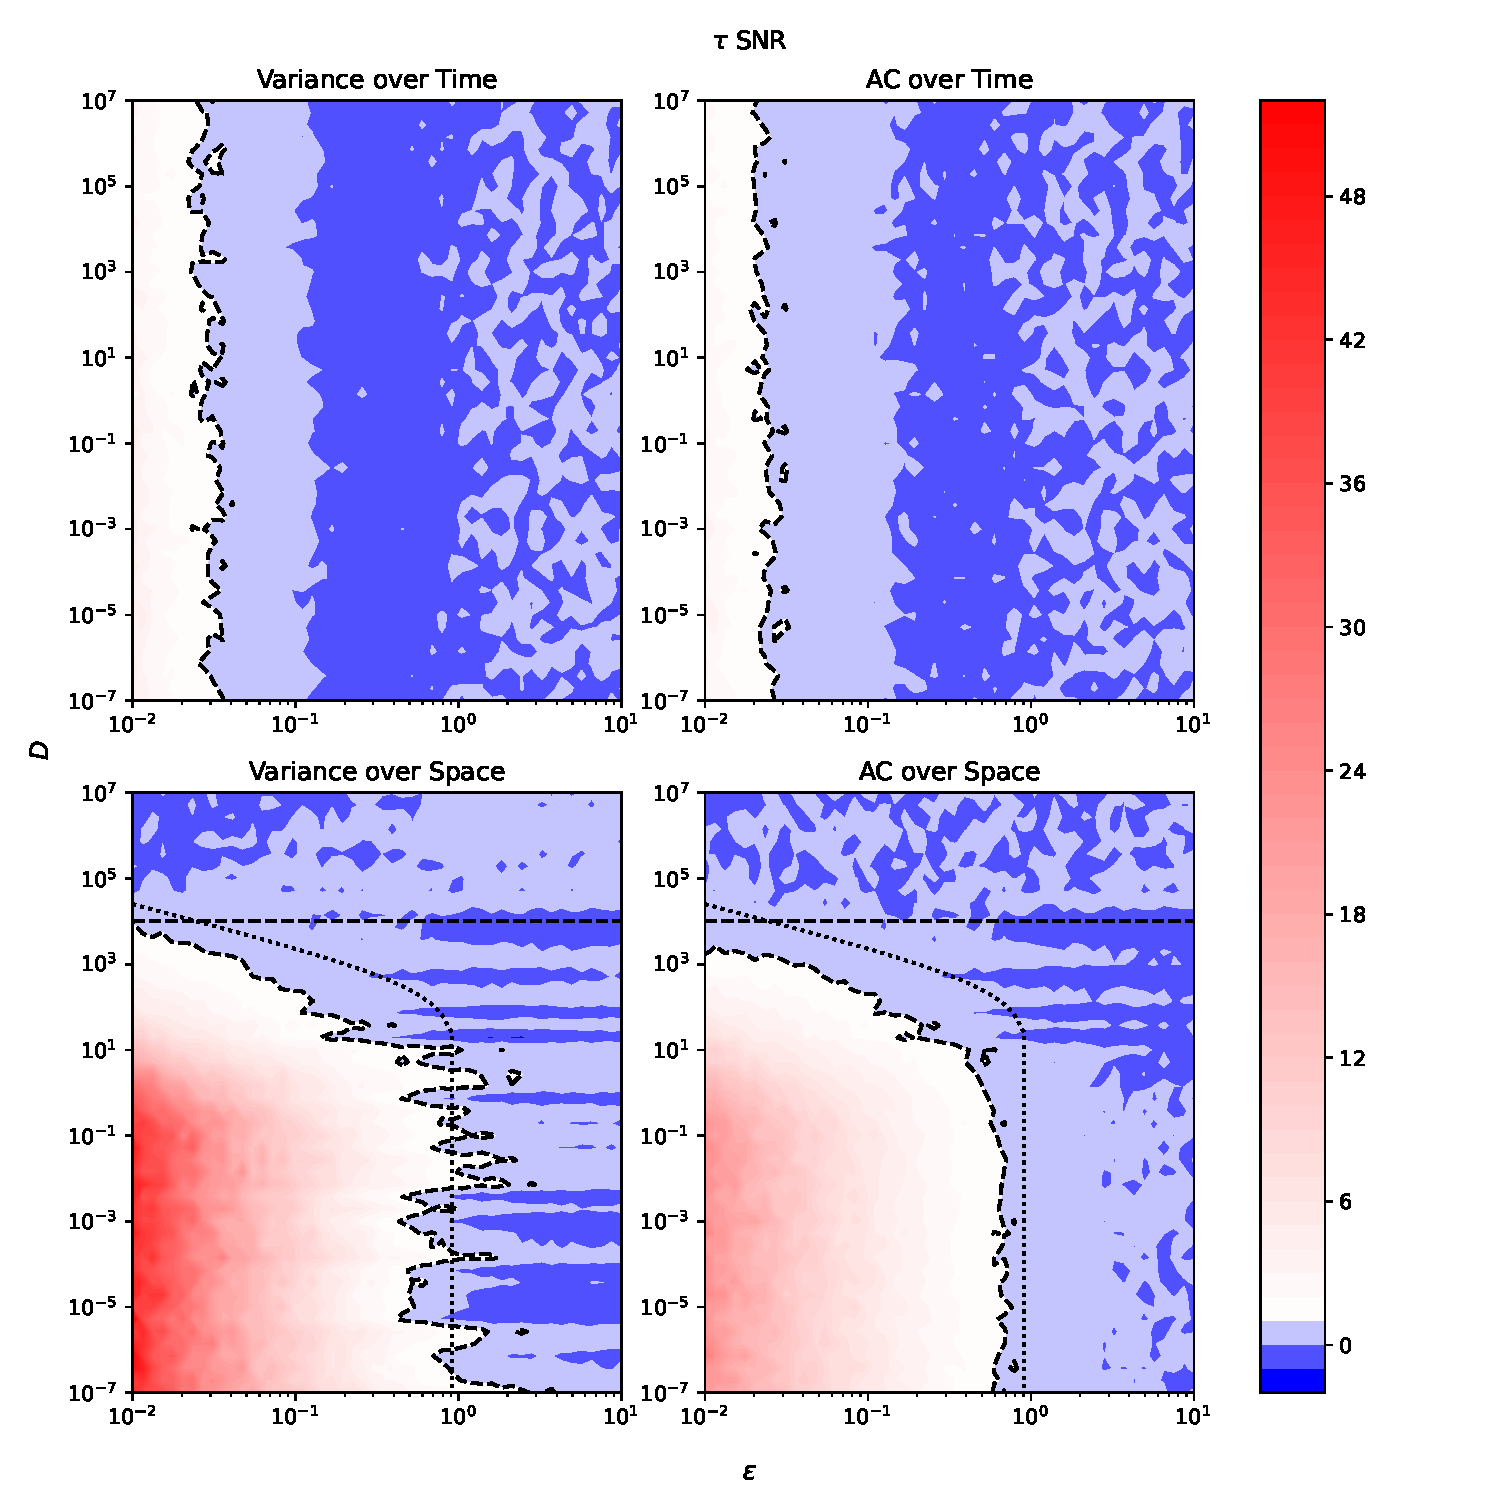
\includegraphics[width=\textwidth,keepaspectratio]{parameter_plane}
  \caption[The quality of early warning signals in the $\epsilon$ and $D$ plane]{Each panel shows the same region of the $(\epsilon,D)$ parameter plane. The left column shows the
    reliability of the variance as an early warning and the right column the reliability of the autocorrelation. The top row is calculated over time and the bottom row is calculated over space.
    The colour gives reliability of the early warning. Blue colours correspond to a SNR of less than $1$, and thus an unreliable early warning. Red colours correspond to reliable early warnings.
    The solid line is the $\mathrm{SNR} = 1$ contour. The dashed line is the line $\sqrt{D} + 40\epsilon\sqrt{D} = L$.}
  \label{fig:parameter_plane}
\end{figure}


\section{Scaling Arguments}
\label{sec:scaling_arguments}
    
In this section an attempt is made to explain why the early warning signals only work in certain regions of the parameter plane plotted in \cref{fig:parameter_plane}.

\subsection{Temporal Early Warning Signals}
Consider the equilibrium solution to \cref{eq:spatial_system_y_variational} (i.e.\ at fixed $\mu$). This will correspond to a minimum
of \cref{eq:spatial_system_energy}. Noting that \cref{eq:spatial_system_energy} is a strictly increasing function of $\pdv*{y}{x}$ it must be the case
that the equilibrium solution is uniform in $x$ and hence independent of $D$.

This motivates setting $y = y_{\mathrm{eq}} + z$ where $y_{\mathrm{eq}}$ is the equilibrium solution to \cref{eq:spatial_system_y_variational}. Temporal
early warning signals are based on $\langle y \rangle$ so its evolution equation will be determined by averaging \cref{eq:spatial_system} in space.
This gives
\begin{align*}
  \dv{\langle y \rangle}{t} &= \langle y \rangle - \frac{1}{3} \left\langle y^3 \right\rangle - \mu + D \left\langle \pdv[2]{y}{x} \right\rangle + \sigma \eta \\
                            &= \langle y \rangle - \frac{1}{3} \left\langle y^3 \right\rangle - \mu + \sigma \eta
\end{align*}
where $\eta$ is noise delta correlated in time only. The diffusive term has vanished due to the periodic boundary conditions. Although there is no explicit dependence on $D$ here,
this equation still implicitly depends on $D$ through the nonlinear averaged term $\left\langle y^3 \right\rangle$.

The evolution equation for $z = y - y_{\mathrm{eq}}$  can be written, to first order in $z$, as
\begin{equation}
  \label{eq:averaged_linear_perturbation_evolution}
  \dv{\langle z\rangle}{t} = \left(1 - y_{\mathrm{eq}}^2\right)\left\langle z \right \rangle + \sigma \eta  + \mathcal{O}\left(z^2 \right)
\end{equation}
where the fact that $y_{\mathrm{eq}}$ is an equilibrium solution of \cref{eq:spatial_system_y} has been used. This has no dependence on
$D$ and hence it can be expected that the temporal early warning signals are independent of $D$.

To get good early warning signals it is required that $\langle z\rangle$ is small so that the linearisation in
\cref{eq:averaged_linear_perturbation_evolution} is valid, but as $z$ is $\mathcal{O}\left(\epsilon^{1/3}\right)$ \parencite{Berglund2006},
good temporal early warning signals can only be expected therefore when $\epsilon^{1/3} \ll 1$.

\subsection{Spatial Early Warning Signals}
It was shown in \cref{sec:spatial_csd} that by recognising the connection between \cref{eq:spatial_system_y_variational} and Landau theory for phase transitions, the two point
correlation function could be computed and the correlation length $\xi = \sqrt{D/\lambda}$ determined. In order to detect any spatial variability the system must be sampled over
scales large compared to the correlation length, which means $L \gg \xi$.

The shortest correlation length occurs when $\lambda$ is largest, which occurs at $t = 0$ when $\lambda = 1$. Therefore in order to get good early
warning signals in space it is therefore necessary that $D \ll L^2$ where $L$ is the size of the domain.

If $\epsilon \neq 0$, then the correlation length will change dynamically. To estimate this change, note that $\dot{\xi} = -\frac{1}{2}\sqrt{D}\lambda^{-3/2} \dot{\lambda}$, so that at time $t$
the value of $\xi \approx \sqrt{D} + \frac{1}{2}\sqrt{D}\lambda^{-3/2} \left|\dot{\lambda}\right|t$. Assuming that $\dot{\lambda} = \mathcal{O}(\epsilon)$ when $t=\mathcal{O}(1)$ then it might be expected
that $\xi \approx \sqrt{D} + F \epsilon \sqrt{D}$, where $F$ is a constant, after a short interval of time. In order to get good early warning signals it should be required that $\xi$ does not reach the
size of the domain too quickly so early warning signals should only be expected when $D \ll L^2 \left(1 + F \epsilon\right)^{-1}$.

In order to view the dynamics as oscillations about equilibrium, it must be the case that the forcing timescale, $1/\epsilon$, is small compared to the timescale
of the dynamics $\tau_k$. As $\tau_k$ is an increasing function of $k$, It is necessary that $\epsilon \tau_0 \ll 1$. If this is to hold at the start of the simulation where
$\tau_0 = 1$, spatial early warning signals cannot be expected when $\epsilon = \mathcal{O}(1)$.

\subsection{Comparison With Numerical Experiments}
\Cref{fig:parameter_plane} implies the critical $\epsilon$ above which temporal early warning signals fail is $\epsilon_c \approx 0.04$.
Performing the computation $\epsilon_c^{1/3} = 0.34$ shows that this is indeed compatible with the theory which requires that $\epsilon^{1/3} \ll 1$.
Also plotted in \cref{fig:parameter_plane} is the  line $D = L^2 \left(1 + F \epsilon\right)^{-1}$ with $F = 40$.
This  line bounds the region where spatial early warning signals are reliable as long as $\epsilon$ is not too large.
For large enough $\epsilon$ no early warnings are possible, as expected, as the timescale of forcing relative to the dynamics becomes too fast.

\section{Discussion}
It has been shown that calculating early warning signals over space allows the user to get reliable
signals in a previously inaccessible parameter regime (for larger values of $\epsilon$).  As well
as having this advantage it is also noted further that calculating early warning signals over space avoids 
the problems of detrending. These problems are inherent to the method of calculating early warning signals over
time.

There is a interesting complementarity however between early warnings in space and time. For fast forcing
and weak coupling in space, early warnings in space are reliable but those in time are not. For slow forcing
but strong spatial coupling then early warnings in time are reliable but those in space are not. If the
coupling is weak but the forcing is slow both methods are reliable. There is still an inaccessible parameter
region, for fast forcing and strong spatial coupling. This is illustrated schematically in figure
\cref{fig:idealised_plot}.
\begin{figure}
  \centering
  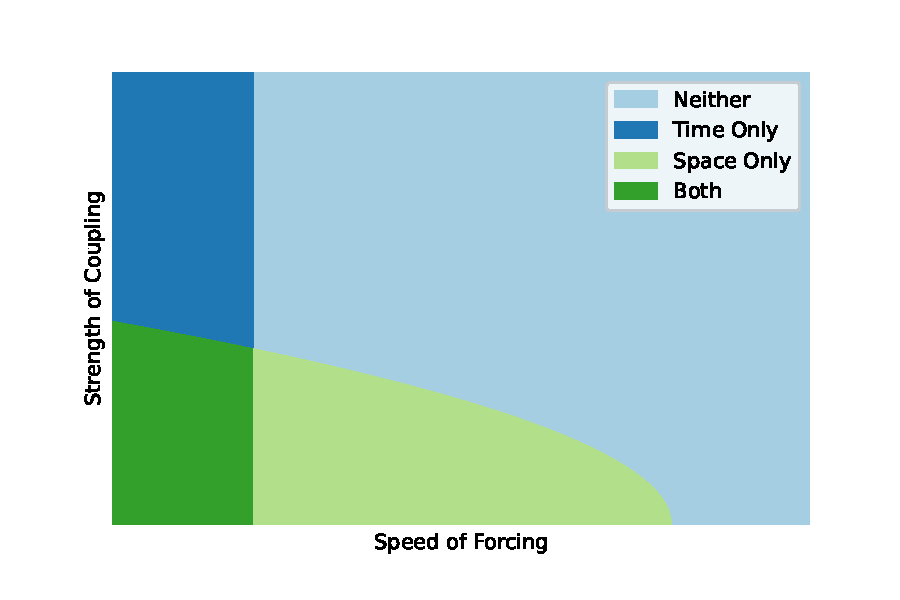
\includegraphics[width=\textwidth,keepaspectratio]{idealised_plot}
  \caption[A schematic showing the complementarity of spatial and temporal early warning signals]{Figure 4: A schematic illustrating the complementarity of early warning signals in space and time.
    The lines are drawn according to the scalings given in \cref{sec:scaling_arguments}}
  \label{fig:idealised_plot}
\end{figure}

\section{Conclusion}

Obtaining temporal early warning signals for tipping points are challenging, not least because they are often used in rapidly forced systems.
In this chapter the hypothesis has been advanced that spatial early warning signals may be useful in these more rapidly forced systems.
It has been found that spatial early warning signals can be used for more rapidly forced systems, as \cref{fig:uncoupled_timeseries,fig:parameter_plane}
illustrate.

It has been shown that their usefulness decreases as the spatial interactions increase.
In particular there is a dichotomy between temporal early warning signals (which work well in strongly spatially coupled and slowly temporally forced systems)
and spatial early warning signals (which work well in weakly spatially coupled and strongly temporally forced systems).

It is noted that there is still an inaccessible parameter region --- systems forced strongly in time and strongly coupled in space. There are also further limitations
to this approach.  Only considered one functional form of coupling has been considered, but others are possible. Secondly, a strong assumption has been made that space is isotropic,
but if, for example, $D$ is itself a function of $x$ then this will introduce challenges.

There is no reason for only one method calculating early warning signal to be used. It is likely that using spatial early warning signals in conjunction with
temporal ones could provide a useful tool to detect approaching tipping points.